\chapter{Introduction}
\label{ch:into} 

%%%%%%%%%%%%%%%%%%%%%%%%%%%%%%%%%%%%%%%%%%%%%%%%%%%%%%%%%%%%%%%%%%%%%%%%%%%%%%%%%%%


\section{Background}
Forest fires represent a significant threat to ecosystems, human lives, and infrastructure worldwide. These catastrophic events result in immediate devastation and long-term environmental and socioeconomic impacts [4]. Forest fires' increasing frequency and severity, particularly in regions with hot, dry climates, have underscored the urgency of developing effective prediction and management strategies [5]. Understanding the factors contributing to forest fire occurrence and progression is essential for mitigating risks and minimizing damages.

%%%%%%%%%%%%%%%%%%%%%%%%%%%%%%%%%%%%%%%%%%%%%%%%%%%%%%%%%%%%%%%%%%%%%%%%%%%%%%%%%%%

\section{Problem Statement}
The challenge of accurately predicting forest fires lies in the complex interactions between various environmental factors, including weather conditions, vegetation types, and human activities. Conventional prediction systems often rely on extensive monitoring features and weather prediction mechanisms, which can be costly and impractical, especially for developing countries. Furthermore, weather prediction inaccuracies can lead to fire risk assessment errors [2]. Therefore, there is a pressing need for cost-effective and efficient forest fire prediction methods that can reliably estimate fire occurrence and progression.

%%%%%%%%%%%%%%%%%%%%%%%%%%%%%%%%%%%%%%%%%%%%%%%%%%%%%%%%%%%%%%%%%%%%%%%%%%%%%%%%%%%

\section{Aims and Objectives}
The primary aim of this study is to investigate and evaluate machine learning techniques for forest fire prediction, focusing on enhancing prediction accuracy and efficiency. The specific objectives of the project are as follows:
\begin{itemize}
     
    \item Review and analyze existing forest fire prediction methodologies, including traditional systems and artificial intelligence-based approaches [4].
    \item To assess the performance of the developed models using real-world forest fire data and evaluate their effectiveness in predicting fire occurrence and progression [5].

\end{itemize}

%%%%%%%%%%%%%%%%%%%%%%%%%%%%%%%%%%%%%%%%%%%%%%%%%%%%%%%%%%%%%%%%%%%%%%%%%%%%%%%%%%%

\section{Solution Approach}
This project adopts a comprehensive approach to address the challenges associated with forest fire prediction. The methodology involves:
\begin{itemize}
    \item Reviewing relevant literature on forest fire prediction methods and machine learning techniques.
    \item Implementing and fine-tuning machine learning models based on the identified methodologies.
    \item Collecting and prepossessing real-world forest fire data for model training and evaluation.
    \item Analysing the performance of the developed models and comparing them with existing prediction systems.
\end{itemize}

\section{Table}
\begin{figure}
    \centering
    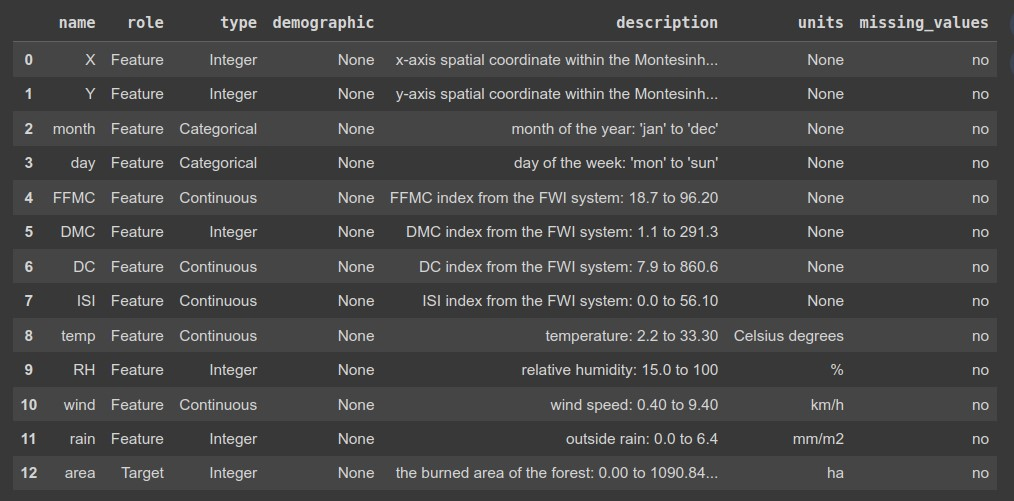
\includegraphics[scale=0.6]{figures/Summary data set.jpg}
    \caption{Table 1: Variable Description : Summarizes dataset variables with names, roles, types, demographics, descriptions, units, and information about missing values. Includes features such as spatial coordinates, meteorological indices, and target variable for burned forest area.}
\end{figure}


%%%%%%%%%%%%%%%%%%%%%%%%%%%%%%%%%%%%%%%%%%%%%%%%%%%%%%%%%%%%%%%%%%%%%%%%%%%%%%%%%%

\section{Summary of contribution and achievements}
This paper contributes to the field of forest fire prediction by exploring various artificial intelligence-based methods and their applications. Specifically, it examines the genetic programming in predicting forest fire occurrences and estimating the extent of burned areas. By analyzing existing literature and conducting experiments, this paper provides insights into the strengths and limitations of different prediction models, offering valuable guidance for future research and practical implementation.


%%%%%%%%%%%%%%%%%%%%%%%%%%%%%%%%%%%%%%%%%%%%%%%%%%%%%%%%%%%%%%%%%%%%%%%%%%%%%%%%%%%

\section{Organization of the report} 
The report starts with an Introduction where we discuss the topic's background, explain the problem we're trying to solve, outline our goals, and describe how we plan to solve the problem. Then, we have a Literature Review section where we review what others have written about our topic and explain how we've cited their work. The Methodology section explains the methods we used in our research. The Results section tells you what we learned from our study. Next, in the Discussion and Analysis section, we carefully consider our results, why they're essential, and mention any limitations we encountered. The Conclusions section summarizes the main things we discovered and suggests ideas for future research. Finally, in the Appendices, we include extra stuff like tables or more details for people who want to know more.


%%%%%%%%%%%%%%%%%%%%%%%%%%%%%%%%%%%%%%%%%%%%%%%%%%%%%%%%%%%%%%%%%%%%%%%%%%%%%%%%%%%



